\documentclass[aspectratio=169,10pt]{beamer}
\usepackage{theme/beamerthemepaper}
\usepackage{booktabs}
\usepackage{hyperref}
\hypersetup{colorlinks,urlcolor=accent,linkcolor=ink}

\title[Transfinite game values in infinite chess]{Transfinite game values in infinite chess}
\subtitle{Two papers by Evans, Hamkins and Perlmutter in \emph{Integers}}
\author{Sean Reid and Andrew Shargel}
\institute{Introduction to Proofs, research paper presentation}
\date{December 2026}

\newcommand{\EH}{[EH14]}
\newcommand{\EHP}{[EHP17]}

\begin{document}

\setpresenter{Sean}

\begin{frame}[plain]
  \titlepage
\end{frame}

\begin{frame}{Two papers, one topic}
  \begin{itemize}
    \item \EH\ C.~D.~A.~Evans and J.~D.~Hamkins, \emph{Transfinite game values in infinite chess},
      Integers 14 (2014), paper G2.
    \item \EHP\ C.~D.~A.~Evans, J.~D.~Hamkins and N.~L.~Perlmutter,
      \emph{A position in infinite chess with game value $\omega^4$}, Integers 17 (2017), paper G4.
  \end{itemize}
  \vskip 0.4cm
  The topic is a single question: how long can a lost game of chess be made to last, and what number
  measures that length?
  \vskip 0.4cm
  \footnotesize
  \begin{tabular}{@{}ll@{}}
    \toprule
    Part A, Sean & ordinals, open games, game values, positions worth $\omega$, $\omega^2$, $\omega^3$ \\
    Part B, Andrew & the position worth $\omega^4$, its main line, how the value falls move by move \\
    \bottomrule
  \end{tabular}
\end{frame}

\begin{frame}{Infinite chess}
  \begin{itemize}
    \item The board is $\mathbb{Z}\times\mathbb{Z}$: every square has a neighbour in every direction. No edges, no corners.
    \item The pieces and their moves are the ordinary ones. Pawns never promote, since there is no last rank.
    \item A win is checkmate, which happens at some move. A game that goes on forever is a draw.
    \item No fifty-move rule and no repetition rule. Stalemate still draws.
    \item Positions may have infinitely many pieces. Every position in this talk is described by a rule.
  \end{itemize}
  \vskip 0.3cm
  \flag{assumed} how the pieces move. Nothing else about chess is needed today.
\end{frame}

\begin{frame}{Open games}
  \begin{block}{Definition}
    A two-player game of perfect information is \emph{open for a player} when every play won by that
    player is already won after finitely many moves: there is a finite stage at which the win is decided,
    whatever happens afterwards.
  \end{block}
  \vskip 0.3cm
  \begin{itemize}
    \item Chess is open for white and open for black, because checkmate is a fact about one position.
    \item A draw by infinite play is not decided at any finite stage. That is why the theory is one-sided:
      we assign numbers to positions from white's point of view, then separately from black's.
    \item Everything below works for any open game. Chess is only where the examples live.
  \end{itemize}
\end{frame}

\begin{frame}{Counting past the natural numbers}
  \[
    0,\ 1,\ 2,\ 3,\ \ldots\quad \omega,\ \omega+1,\ \omega+2,\ \ldots\quad
    \omega\cdot 2,\ \ldots\quad \omega\cdot 3,\ \ldots\quad \omega^2,\ \ldots\quad \omega^3,\ \ldots\quad \omega^4
  \]
  \begin{itemize}
    \item The \emph{ordinals} extend the naturals. $\omega$ comes after every natural number.
      $\omega+1$ comes after $\omega$. $\omega\cdot 2$ comes after every $\omega+n$, and so on.
    \item Every ordinal $\alpha$ has a next one, $\alpha+1$. Some ordinals, like $\omega$ and $\omega^2$, are
      \emph{limits}: they have no immediate predecessor.
    \item $\omega^3\cdot 5+\omega^2\cdot 7+\omega+14$ is an ordinal. Compare two such sums by their leading term,
      then the next, as with decimal digits.
  \end{itemize}
  \begin{alertblock}{The one fact we use}
    There is no infinite strictly decreasing sequence of ordinals.
    Reason: any nonempty set of ordinals has a least element, and a decreasing sequence would have none.
  \end{alertblock}
\end{frame}

\begin{frame}{A countdown game}
  \flag{our teaching device, not from the papers}
  \vskip 0.2cm
  A counter shows an ordinal. White wins when it shows $0$.
  \begin{itemize}
    \item White moves from a successor $\alpha+1$ to $\alpha$.
    \item Black moves at a limit: from $\lambda$, black may choose any ordinal below $\lambda$.
  \end{itemize}
  \vskip 0.2cm
  {\small
  \begin{tabular}{@{}lll@{}}
    \toprule
    start & what black gets to do & length of the game \\
    \midrule
    $n$ & nothing & exactly $n$ white moves \\
    $\omega$ & announce one natural $n$ & $n$, any finite length black likes \\
    $\omega\cdot 2$ & announce $n$, later announce $m$ & $n+m$, two free choices \\
    $\omega^2$ & announce $n$: the number of later announcements & $n$ rounds, each as long as black likes \\
    \bottomrule
  \end{tabular}}
  \vskip 0.2cm
  White always wins, by the fact on the last slide. Black controls how long it takes, and the ordinal
  says exactly how much control black has.
\end{frame}

\begin{frame}{Game value: the definition}
  Fix white as the designated player. Values are ordinals, assigned to positions by recursion.
  \begin{block}{Definition (\EH, Definition 1; \EHP, Section 2)}
    \begin{itemize}
      \item A position in which white has already won has value $0$.
      \item If it is white's turn at $p$, then $p$ has value $\alpha+1$ when $\alpha$ is the least ordinal such
        that some legal white move from $p$ reaches a position of value $\alpha$.
      \item If it is black's turn at $p$, then $p$ has a value only if \emph{every} legal black move from $p$
        reaches a position that has a value, and then the value of $p$ is the supremum of those values.
    \end{itemize}
    The valuation is the least assignment obeying these rules. Positions can be left without a value.
  \end{block}
  \vskip 0.2cm
  Finite value $n$: white can mate in $n$ and not faster. Value $\omega$: white wins, and black's first move
  picks a natural $n$ with the game lasting at least $n$ more white moves.
\end{frame}

\begin{frame}{The fundamental observation}
  \begin{block}{Theorem (\EH, Section 2, ``the fundamental observation of game values'')}
    If a position has a value, white has a winning strategy from it.
    If a position has no value, black has a strategy that prevents white from ever winning.
  \end{block}
  \begin{proof}[Proof, first half]
    Suppose $p$ has a value. White plays, at each turn, a move to a position of least value; by the
    successor clause that value is one less. Black, by the supremum clause, can never move to a position of
    larger value or to one without a value. So the values along the play strictly decrease. By the fact on
    ordinals the play must reach value $0$, a win for white.
  \end{proof}
\end{frame}

\begin{frame}{The fundamental observation, continued}
  \begin{proof}[Proof, second half]
    Suppose $p$ has no value. If it is white's turn, no white move reaches a valued position, otherwise the
    successor clause would have valued $p$. If it is black's turn, some black move reaches an unvalued
    position, otherwise the supremum clause would have valued $p$. Black always plays such a move, and white
    never reaches value $0$.
  \end{proof}
  \vskip 0.3cm
  So the positions with a value for white are exactly the positions white can force to a win, and
  \emph{reduce the value} is the winning strategy. The same holds with the colours swapped.
  \vskip 0.3cm
  \flag{stated} This argument is the proof of the Gale--Stewart theorem (1953): every open game is determined.
\end{frame}

\begin{frame}{Worked example: a position with value $\omega$}
  \begin{columns}[T]
    \begin{column}{0.3\textwidth}
      \fig[\textwidth]{eh14-fig3}
      \credit{Figure 3 of \EH.}
    \end{column}
    \begin{column}{0.66\textwidth}
      Black to move; the claim is value exactly $\omega$.
      \begin{itemize}
        \item Black lifts the centre rook to any height; white rolls the king up with checks:
          \coord{1...Re10 2.Rf5+ Ke6 3.Qd5+ Ke7 4.Rf7+ Ke8 5.Qd7+ Ke9 6.Rf9\#}.
        \item Height $n$ buys about $n$ white moves: finite but unbounded values, supremum $\omega$.
        \item Any other first move loses at once, for example \coord{1...Rf6 2.Re4+ Kf5 3.Qd5\#}.
        \item White has nothing faster: skewering the lifted rook lets the king out of the net.
      \end{itemize}
      \flag{proof sketch} following the paper's analysis; the exhaustive move check is not written out.
    \end{column}
  \end{columns}
\end{frame}

\begin{frame}{Worked example: a position with value $\omega^2$}
  \begin{columns}[T]
    \begin{column}{0.4\textwidth}
      \fig[\textwidth]{eh14-fig7}
      \credit{Figure 7 of \EH.}
    \end{column}
    \begin{column}{0.56\textwidth}
      \begin{itemize}
        \item The pawn column splits the plane. The marked pawn is a portcullis: once it moves, the
          queens pour through and mate.
        \item Black lifts the centre rook to height $n$; white must push the column $n$ times to free the
          bishop holding the door.
        \item After each push, black's free rook checks the white king from a distance $k$ of black's
          choosing; after $k$ checks it must retreat, and white pushes again.
        \item Black announces $n$, the number of future announcements of a $k$. That is $\omega^2$.
      \end{itemize}
      \flag{proof sketch} the paper argues every deviation shortens the game.
    \end{column}
  \end{columns}
\end{frame}

\begin{frame}{From $\omega^2$ to $\omega^3$: rook towers}
  \begin{columns}[T]
    \begin{column}{0.52\textwidth}
      \fig[\textwidth]{eh14-fig10}
      \credit{Figure 10 of \EH, a position with value $\omega^3$.}
    \end{column}
    \begin{column}{0.44\textwidth}
      \begin{itemize}
        \item The attacked bishop at \coord{m6} runs up its diagonal past $k$ towers before it is taken.
          That $k$ is black's first announcement.
        \item Each tower is worth $\omega^2$: a rook lifted to height $n$, and a round of harassing checks
          after every white pawn step. Towers are consumed right to left.
        \item $k$ towers give at least $\omega^2\cdot k$; $k$ is unbounded, so the value is $\omega^3$.
      \end{itemize}
    \end{column}
  \end{columns}
\end{frame}

\begin{frame}{What the 2014 paper proves, and what it asks}
  \begin{itemize}
    \item \flag{proved in \EH} Positions with values $\omega$, $\omega^2$, $\omega^2\cdot k$ for every $k$, and $\omega^3$
      exist (Section 3 of \EH).
    \item \flag{defined} The \emph{omega one of chess} is the supremum of the values of all positions:
      $\omega_1^{\mathfrak{Ch}}$ over finite positions, $\omega_1^{\mathfrak{Ch}}$ with a tilde over all positions.
    \item \flag{stated, not proved here} Theorem 4 of \EH: $\omega_1^{\mathfrak{Ch}}\le\omega_1^{\mathrm{CK}}$,
      the Church--Kleene ordinal, and the boldface version is at most $\omega_1$. Every value of a winning
      position is a countable ordinal.
    \item \flag{conjecture} Conjecture 5 of \EH: both bounds are sharp.
    \item \flag{stated} Theorem 10 of \EH: in infinite three-dimensional chess every countable ordinal is a value.
  \end{itemize}
  \vskip 0.3cm
  Before 2015 the largest value known in ordinary infinite chess was $\omega^3$, with a sketch reaching
  $\omega^3\cdot 4$. The second paper raises the record to $\omega^4$.
\end{frame}

\setpresenter{Andrew}

\begin{frame}{The theorem}
  \begin{block}{Theorem 1 of \EHP}
    There is a position in infinite chess with game value $\omega^4$. The position is computable and involves
    infinitely many pieces.
  \end{block}
  \vskip 0.3cm
  \begin{itemize}
    \item \emph{Position}: an assignment of pieces to squares of $\mathbb{Z}\times\mathbb{Z}$, with black to move.
    \item \emph{Computable}: a program decides what sits on any given square.
    \item \emph{Value $\omega^4$}: white wins, and black's choices along the way count down from $\omega^4$ in the
      sense of the countdown game: four nested kinds of announcement.
  \end{itemize}
\end{frame}

\begin{frame}{The position}
  \fig[\textwidth]{ehp17-fig1}
  \credit{Figure 1 of \EHP.}
  \begin{columns}[T]
    \begin{column}{0.32\textwidth}
      Throne room, upper left. Both kings, locked in. Whoever frees a bishop mates.
    \end{column}
    \begin{column}{0.32\textwidth}
      Rook towers, running to the upper right. White's slow main attack.
    \end{column}
    \begin{column}{0.32\textwidth}
      Bishop cannon battery, lower half. Black's source of forced replies.
    \end{column}
  \end{columns}
\end{frame}

\begin{frame}{The throne room}
  \begin{columns}[T]
    \begin{column}{0.3\textwidth}
      \fig[\textwidth]{ehp17-fig2}
      \credit{Figure 2 of \EHP.}
    \end{column}
    \begin{column}{0.66\textwidth}
      \begin{itemize}
        \item Nothing here can move. Both kings are exposed to a bishop of the right colour.
        \item A white bishop on the marked diagonal mates at once, for instance \coord{1.Bc10\#}.
        \item A black bishop arriving on its diagonal needs three more moves:
          \coord{1...Bc11 2...Bg7 3...Bj10 4...Bh12\#}.
      \end{itemize}
      \begin{alertblock}{The tempo lemma}
        Black needs three moves after reaching the entry diagonal; a white guard that arrives on its
        diagonal two moves later still mates first. This difference is what makes every gateway attack a
        threat white must answer immediately.
      \end{alertblock}
    \end{column}
  \end{columns}
\end{frame}

\begin{frame}{The rook towers}
  \begin{columns}[T]
    \begin{column}{0.36\textwidth}
      \fig[\textwidth]{ehp17-fig3}
      \credit{Figure 3 of \EHP.}
    \end{column}
    \begin{column}{0.6\textwidth}
      \begin{enumerate}
        \item The key bishop at \coord{f7} is attacked. Black sends it up the diagonal as far as it likes.
          \flag{announcement $r$}: how many towers white must work through.
        \item A white pawn takes it, pierces the wall, and a key pawn attacks the tower's guard pawn.
        \item The attacked rook goes up as high as black likes. \flag{announcement $h$}: how many pawn
          moves white needs to march the hole down.
        \item The hole releases the next tower's bishops and the process repeats one tower to the left.
          The last tower frees the mating bishop.
      \end{enumerate}
      The $\omega^3$ position's structure, minus the harassing rook.
    \end{column}
  \end{columns}
\end{frame}

\begin{frame}{A gateway terminal wing}
  \begin{columns}[T]
    \begin{column}{0.36\textwidth}
      \fig[\textwidth]{ehp17-fig4}
      \credit{Figure 4 of \EHP, a wing of length three.}
    \end{column}
    \begin{column}{0.6\textwidth}
      \begin{itemize}
        \item A black bishop on the entrance diagonal can land on any attack square, each threatening a
          door pawn.
        \item Ignored, black captures, exits, and reaches the throne room three moves ahead of the guard,
          which mates by the tempo lemma.
        \item So white moves the guard one step at once; it then follows two behind, which the lemma says
          is enough.
        \item A wing of length $n$ yields $n+1$ forced replies. \flag{the count $g$}
      \end{itemize}
    \end{column}
  \end{columns}
\end{frame}

\begin{frame}{A bishop cannon}
  \begin{columns}[T]
    \begin{column}{0.3\textwidth}
      \fig[\textwidth]{ehp17-fig5}
      \credit{Figure 5 of \EHP, three shooters.}
    \end{column}
    \begin{column}{0.66\textwidth}
      \begin{itemize}
        \item The shooters are bishops capped by pawns. Moving a capped bishop out uncovers a pawn threat
          that white must meet with a guard pawn, so each shot is a forced reply.
        \item The fired bishop lands on the entrance diagonal of a fresh wing and spends $g$ more forced
          replies there.
        \item Opening a cannon of $n$ shooters costs black one tempo, white's only free move, and buys $n$
          shots. \flag{the count $b$}
        \item Cannons grow without bound along the battery, so black can always open a bigger one.
      \end{itemize}
    \end{column}
  \end{columns}
\end{frame}

\begin{frame}{The value of a main-line position}
  \begin{block}{The value during the main line (\EHP, Section 3)}
    \[
      \omega^3\cdot r \;+\; \omega^2\cdot h \;+\; \omega\cdot b \;+\; g
    \]
    $r$ towers not yet activated, $h$ white moves left in the current tower, $b$ capped shooters left in the
    active cannon, $g$ forced replies left in the active wing.
  \end{block}
  \begin{itemize}
    \item Each black gateway attack lowers $g$ by one. Each shot lowers $b$ by one and raises $g$ by a large
      number. Opening a cannon raises $b$ by a large number but gives white one free move, which lowers $h$.
    \item When $h$ hits zero the next tower activates: $r$ drops by one and black chooses the new $h$.
    \item Black can never raise a leading term. White lowers one every time black lets go of the forced
      replies.
  \end{itemize}
  \flag{proof sketch} the paper's analysis is careful but informal in places; the slide reports its structure.
\end{frame}

\begin{frame}{The value, move by move}
  \flag{supplementary, ours} The next five frames are stills from a browser implementation of the Section 4
  compact position and of white's strategy, written for this presentation. It is not part of the published
  results. \url{https://infinite-chess.dwainosaur.com}
  \vskip 0.3cm
  Each still is the panel after one black move and white's reply. Watch which term moves.
\end{frame}

\begin{frame}{The value, move by move: 1 of 5}
  \framesubtitle{The key bishop goes out three squares}
  \centering
  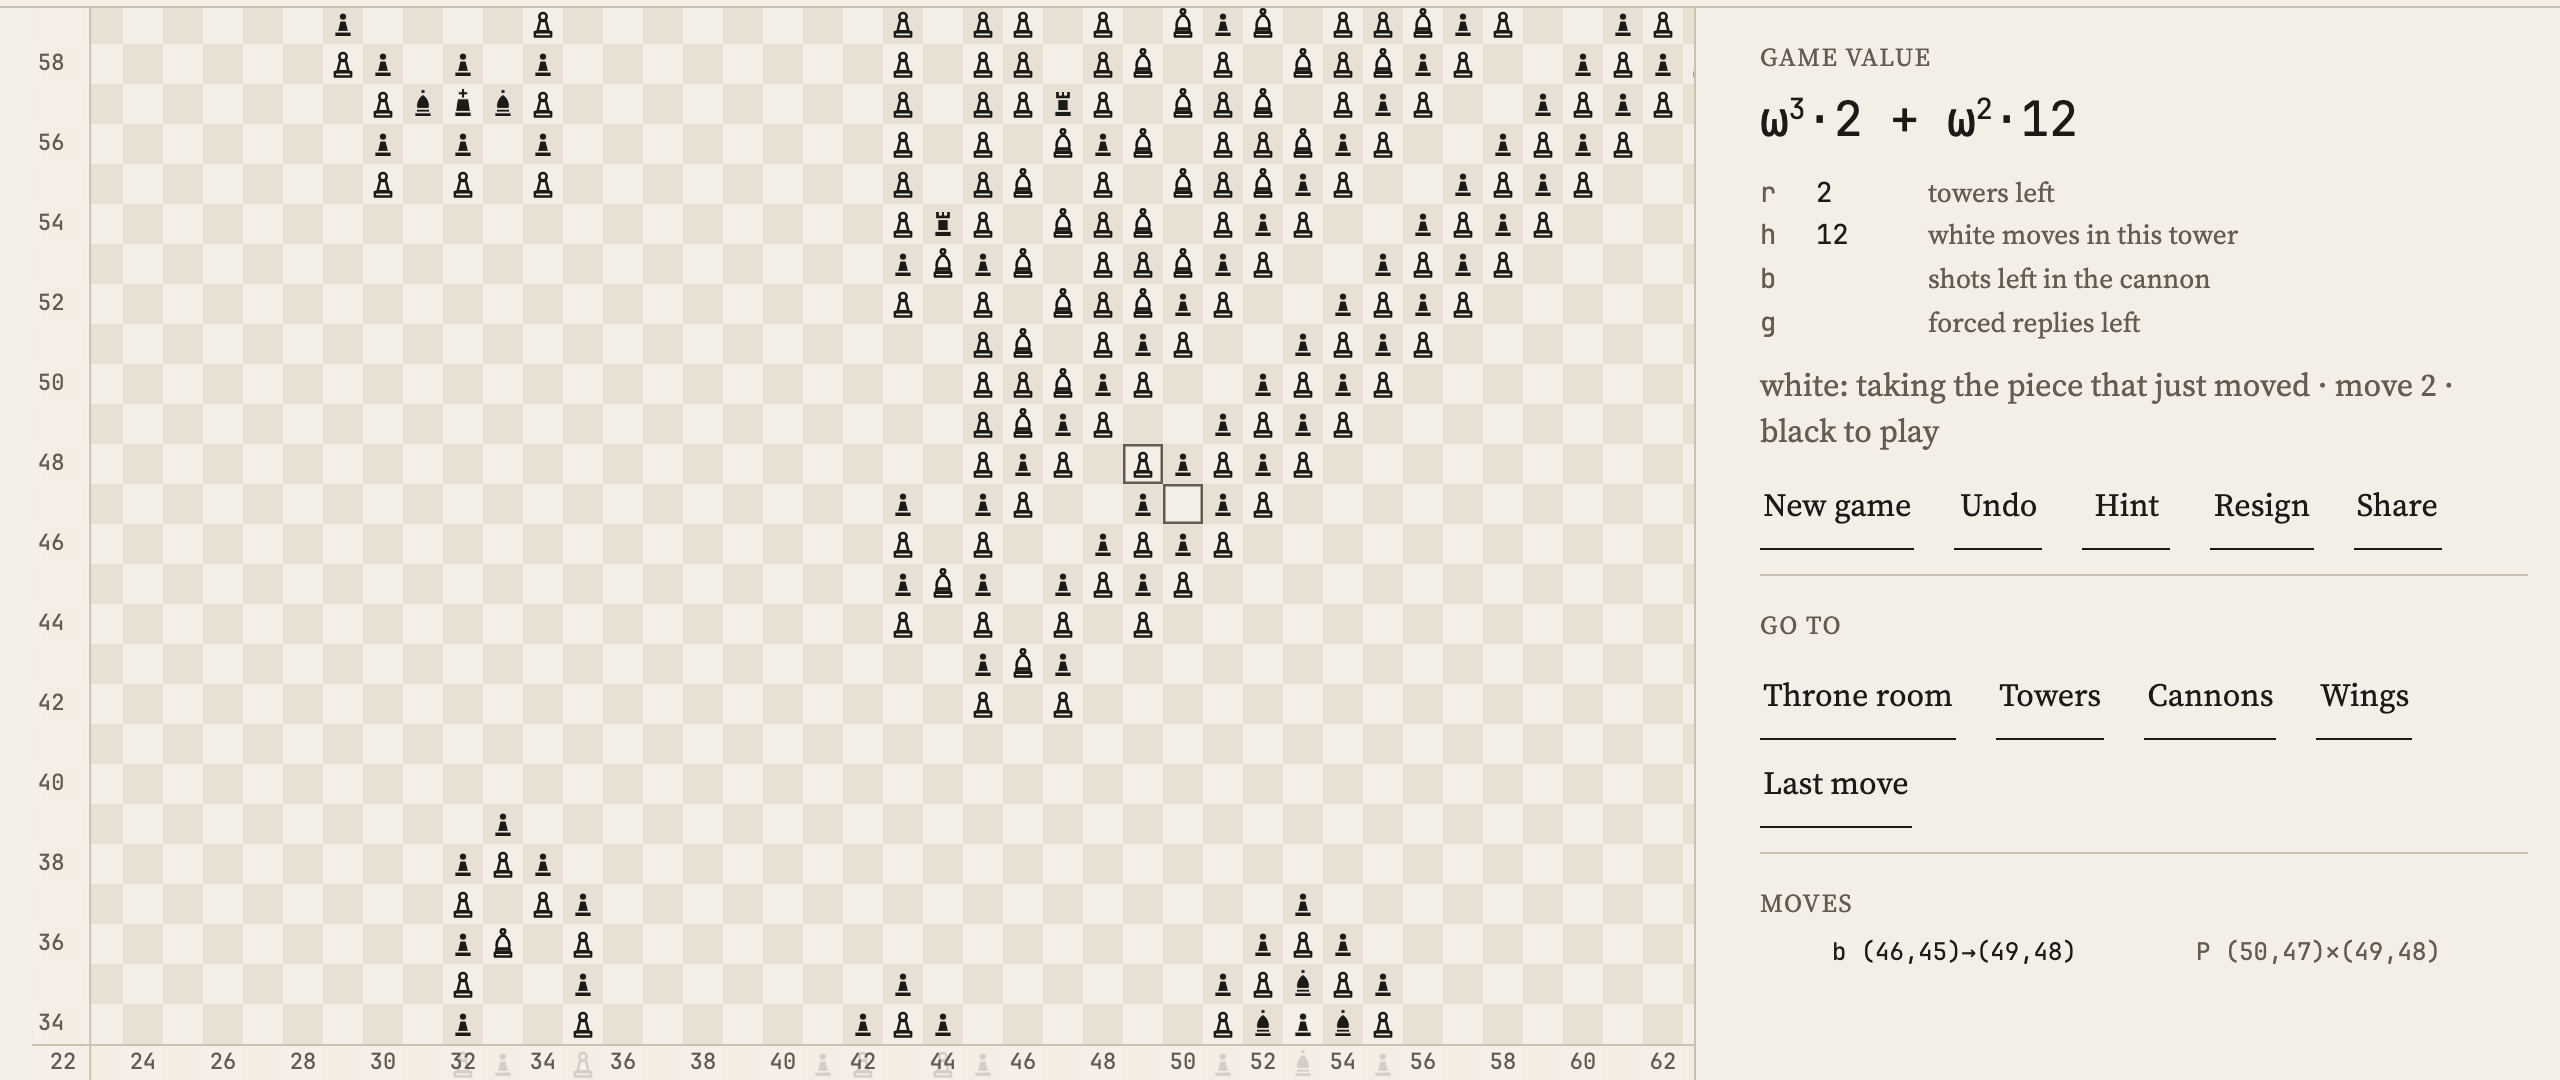
\includegraphics[width=\textwidth,height=0.67\textheight,keepaspectratio]{figures/demo/1-key-bishop.png}
  \par\vskip 0.1cm
  {\footnotesize White takes it: $\omega^3\cdot 2+\omega^2\cdot 12$. The distance chose $r=2$; $h=12$ free moves to go in this tower.}
\end{frame}

\begin{frame}{The value, move by move: 2 of 5}
  \framesubtitle{Black opens cannon 1 at wing 1}
  \centering
  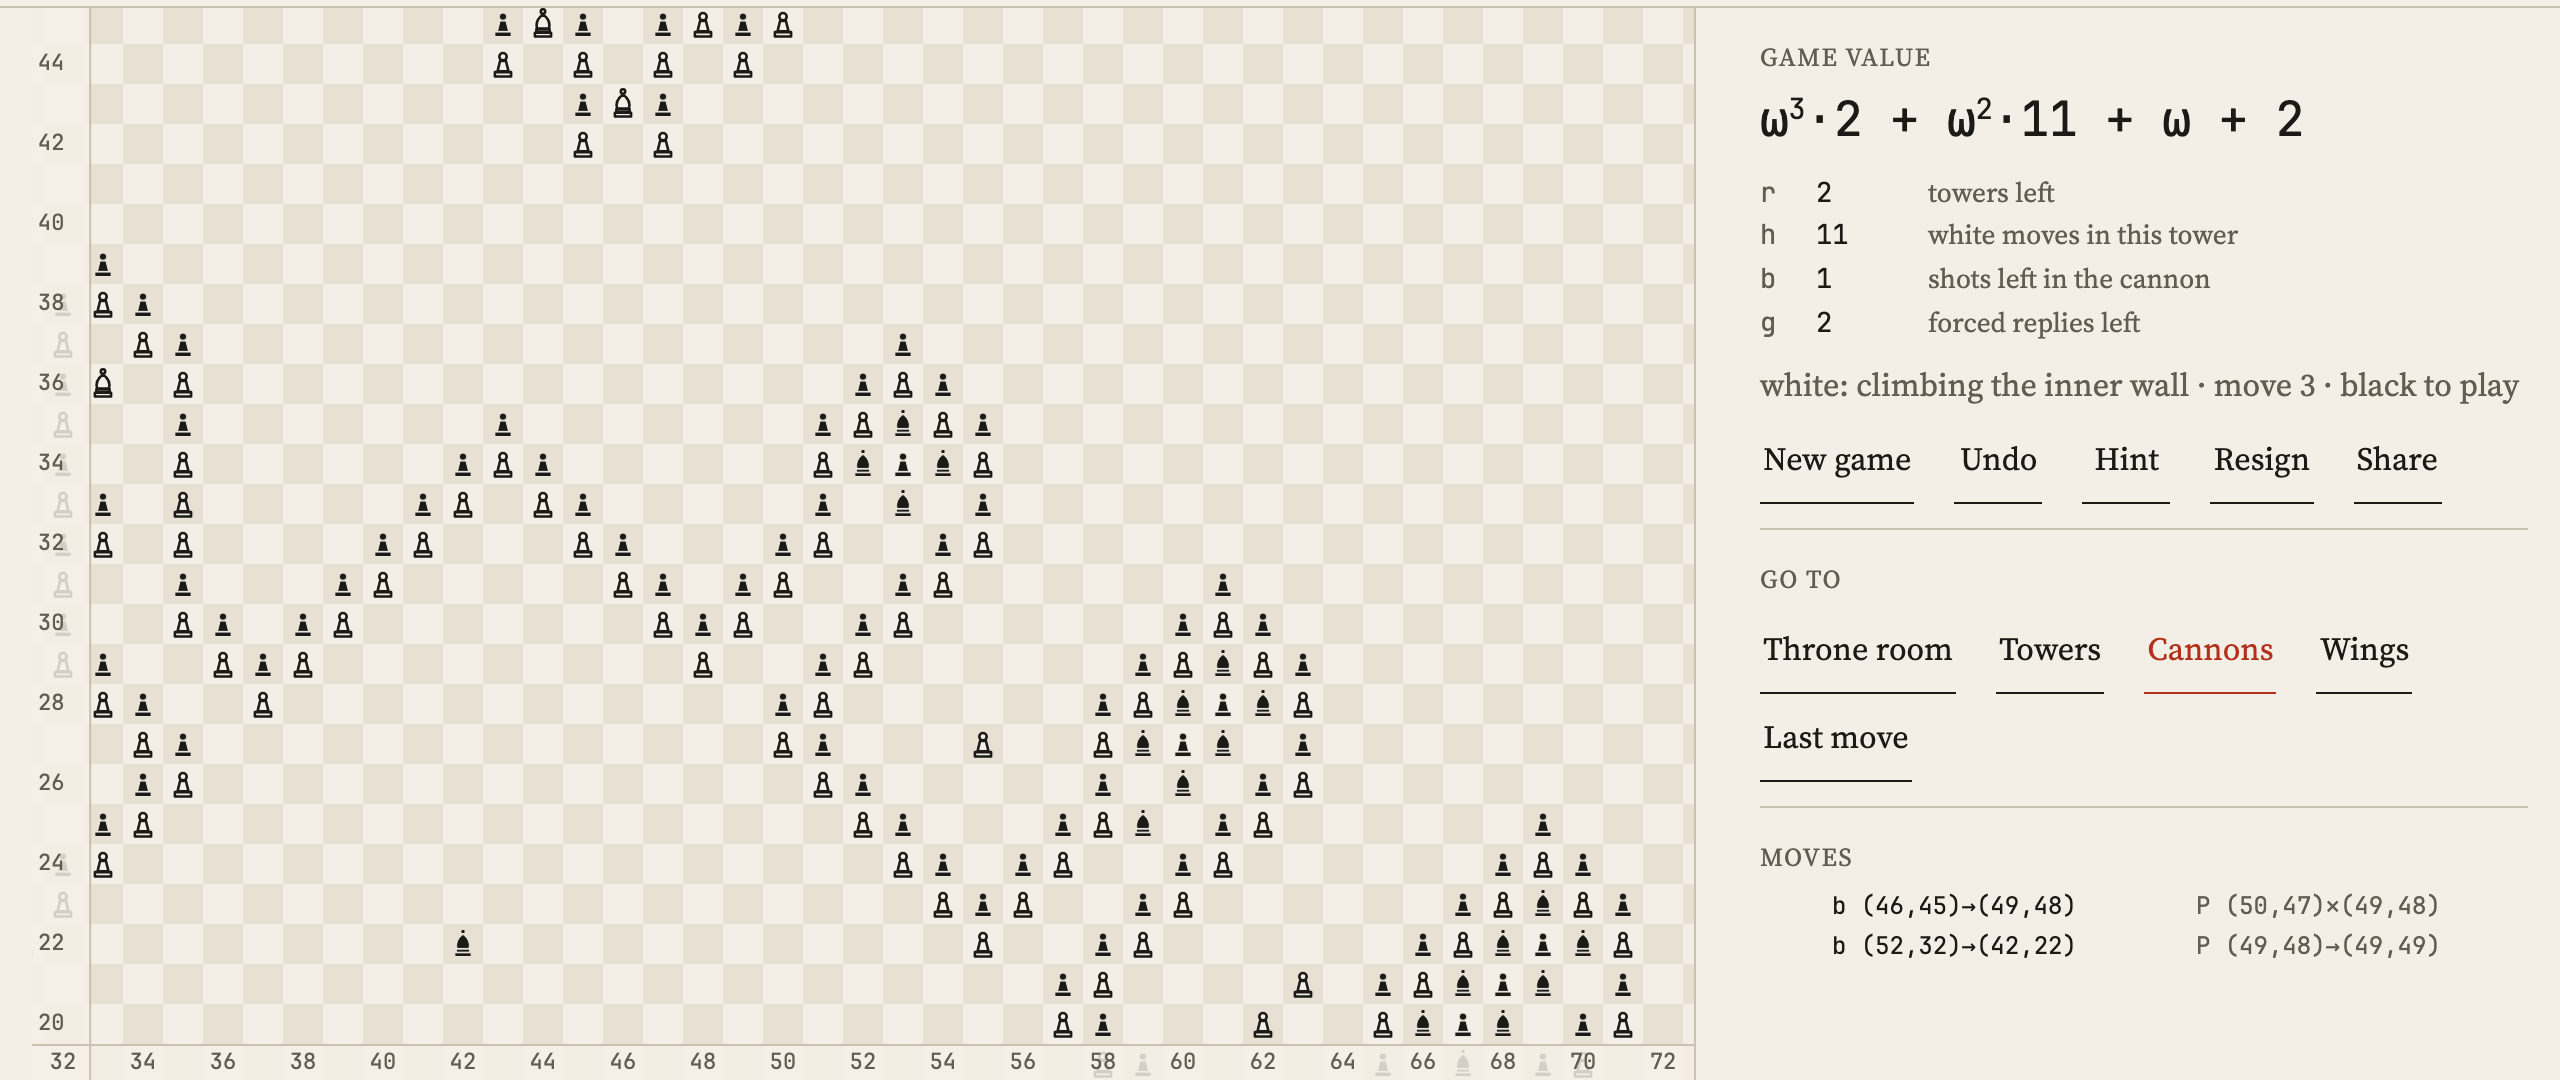
\includegraphics[width=\textwidth,height=0.67\textheight,keepaspectratio]{figures/demo/2-cannon-open.png}
  \par\vskip 0.1cm
  {\footnotesize $b$ and $g$ appear, and white's one free move took $h$ from 12 to 11: $\omega^3\cdot 2+\omega^2\cdot 11+\omega+2$.}
\end{frame}

\begin{frame}{The value, move by move: 3 of 5}
  \framesubtitle{The bishop attacks gate 1; white answers}
  \centering
  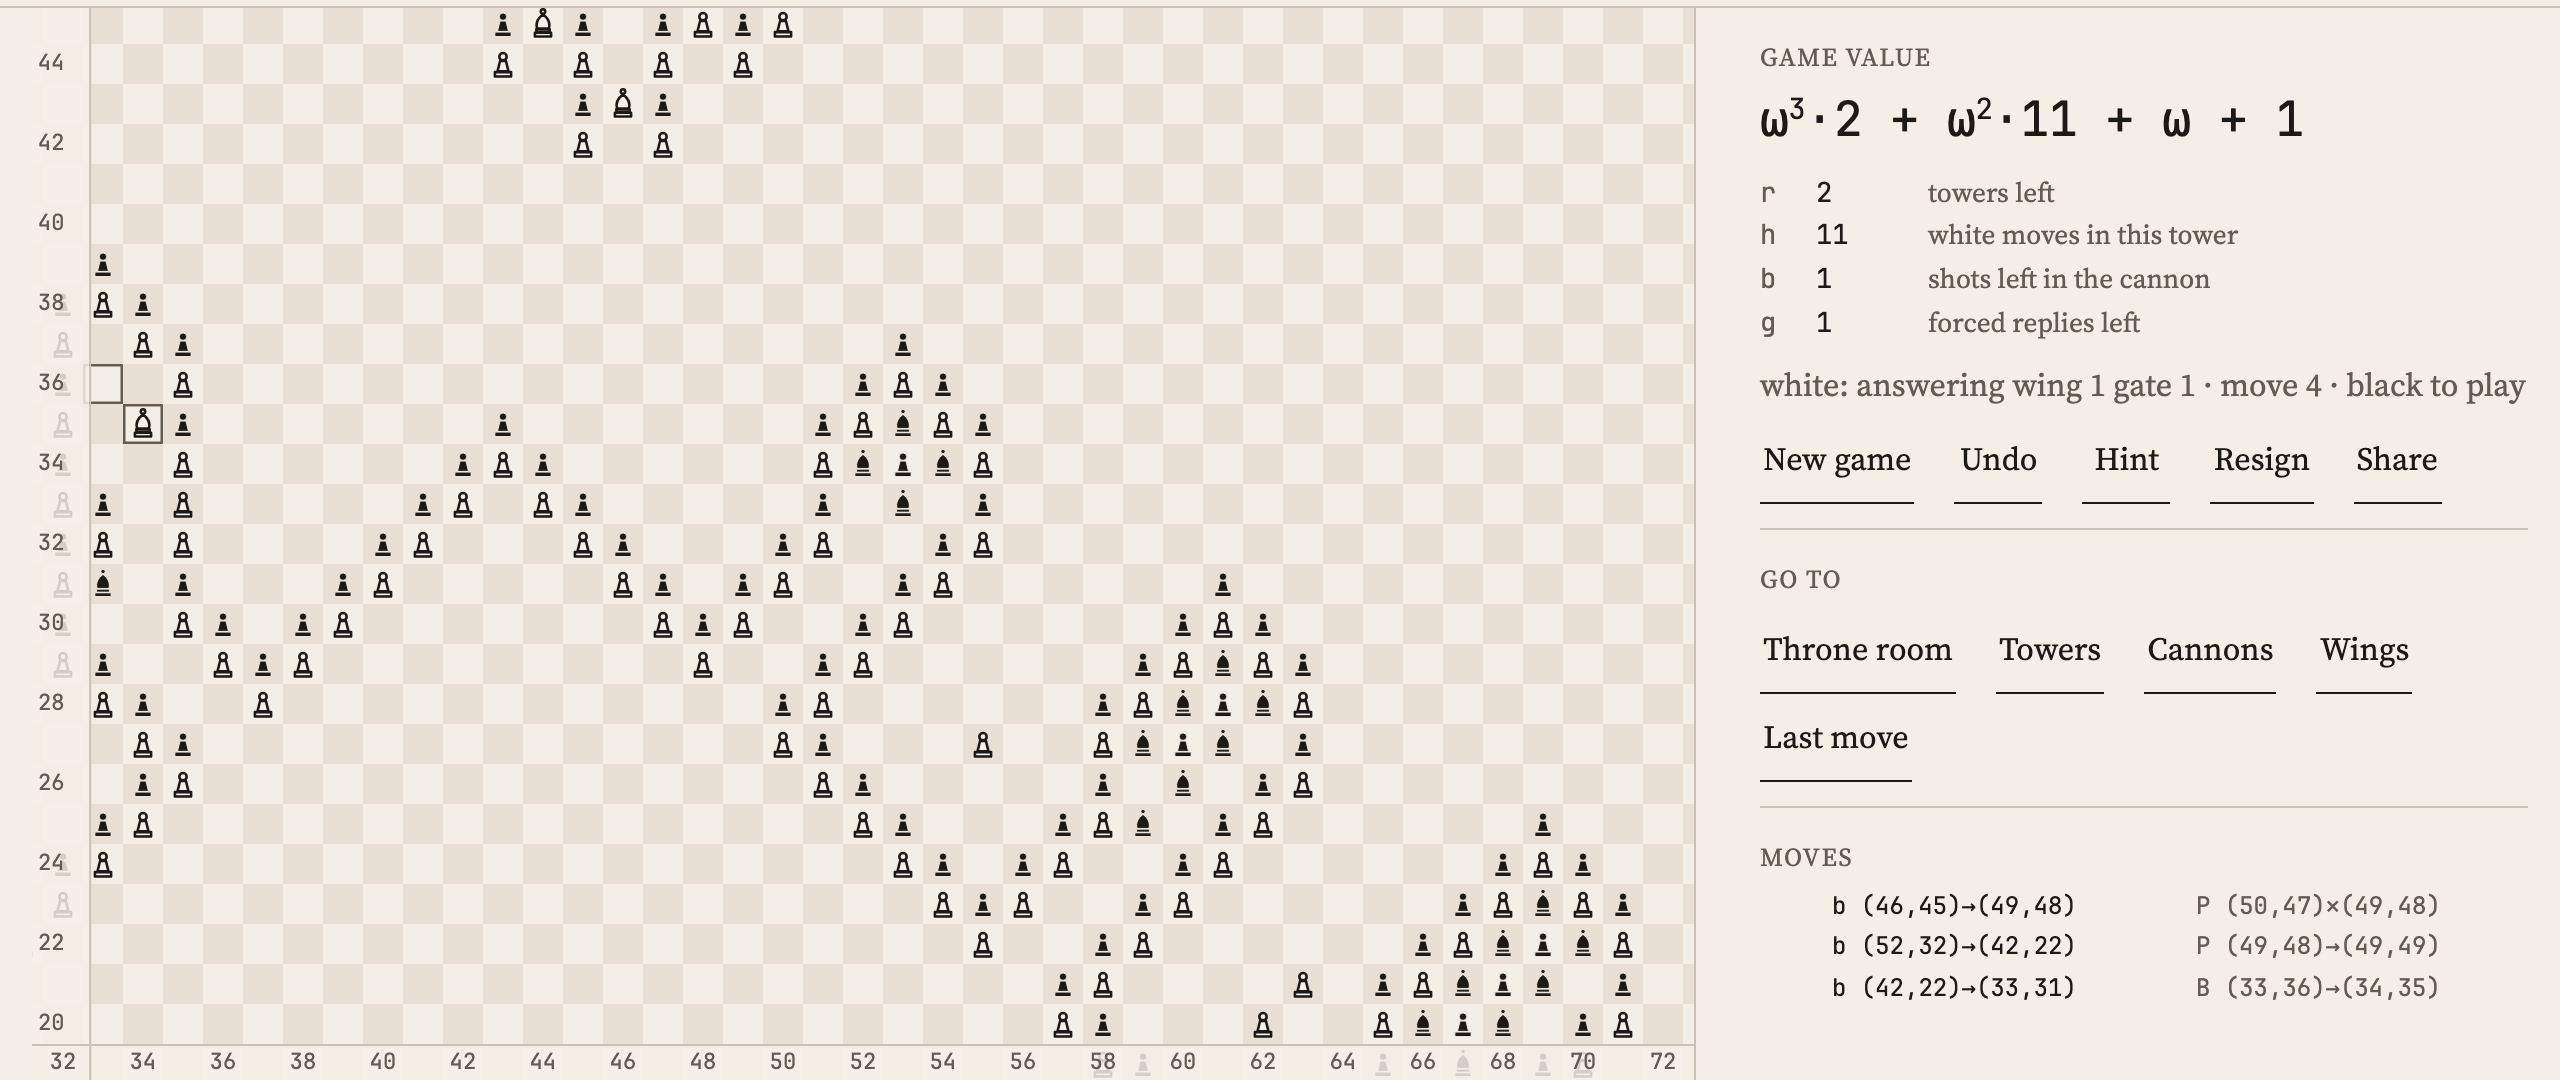
\includegraphics[width=\textwidth,height=0.67\textheight,keepaspectratio]{figures/demo/3-gate-answered.png}
  \par\vskip 0.1cm
  {\footnotesize A forced reply: $g$ went from 2 to 1 and nothing else moved: $\omega^3\cdot 2+\omega^2\cdot 11+\omega+1$.}
\end{frame}

\begin{frame}{The value, move by move: 4 of 5}
  \framesubtitle{Shooter 1 fires at wing 2}
  \centering
  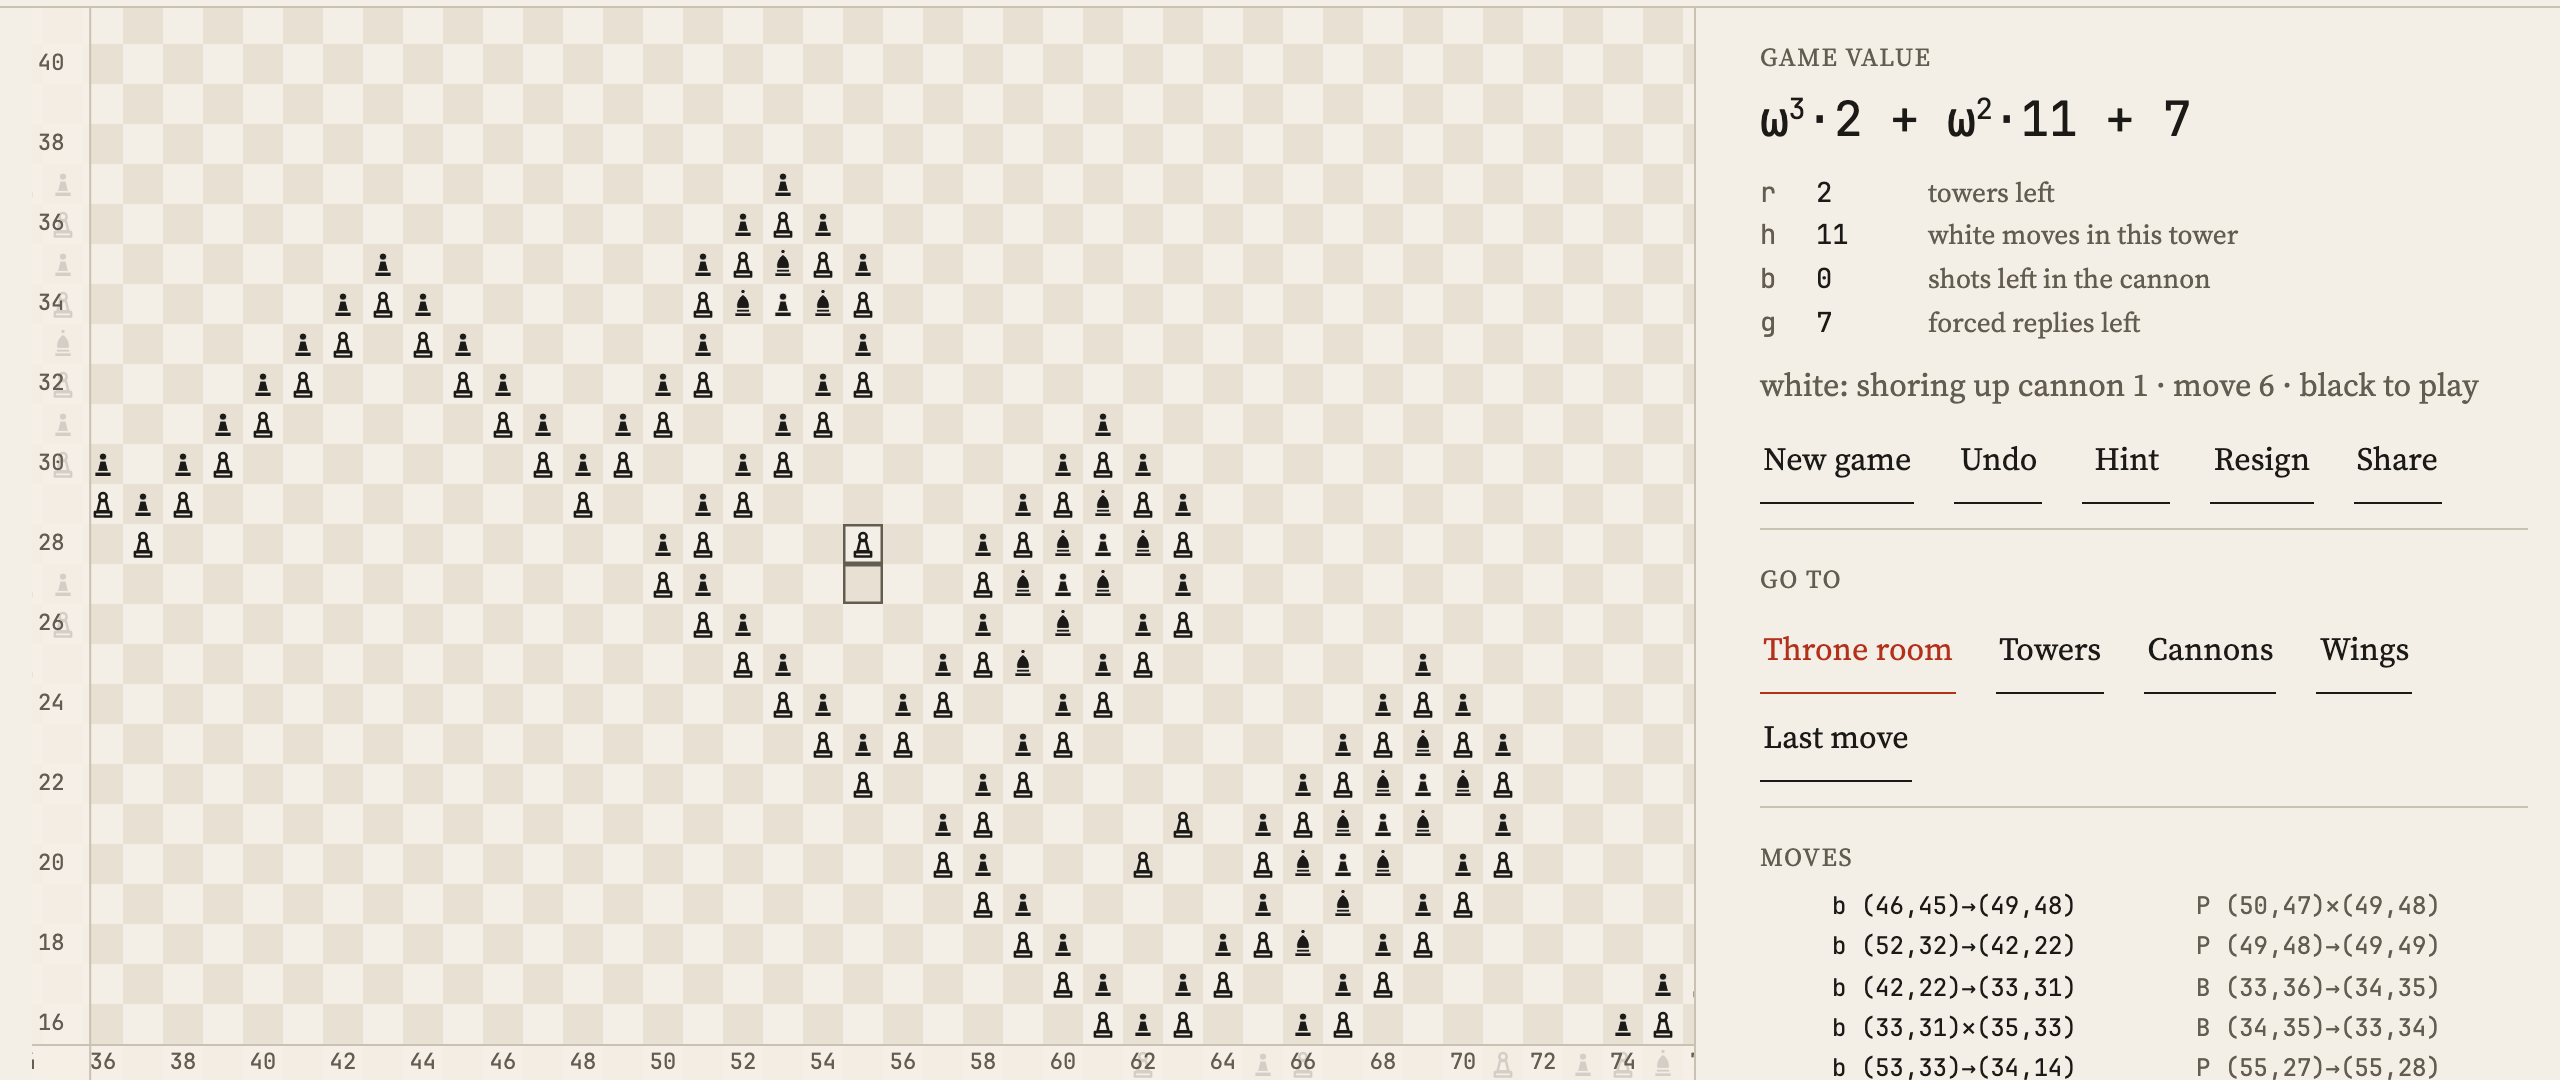
\includegraphics[width=\textwidth,height=0.67\textheight,keepaspectratio]{figures/demo/4-shot.png}
  \par\vskip 0.1cm
  {\footnotesize $b$ fell to 0 and $g$ jumped to 7 as the shot reached a fresh wing: $\omega^3\cdot 2+\omega^2\cdot 11+7$.}
\end{frame}

\begin{frame}{The value, move by move: 5 of 5}
  \framesubtitle{Six hundred plies on, the rook goes up five and is taken: $\omega^3+\omega^2\cdot 13+\omega$}
  \centering
  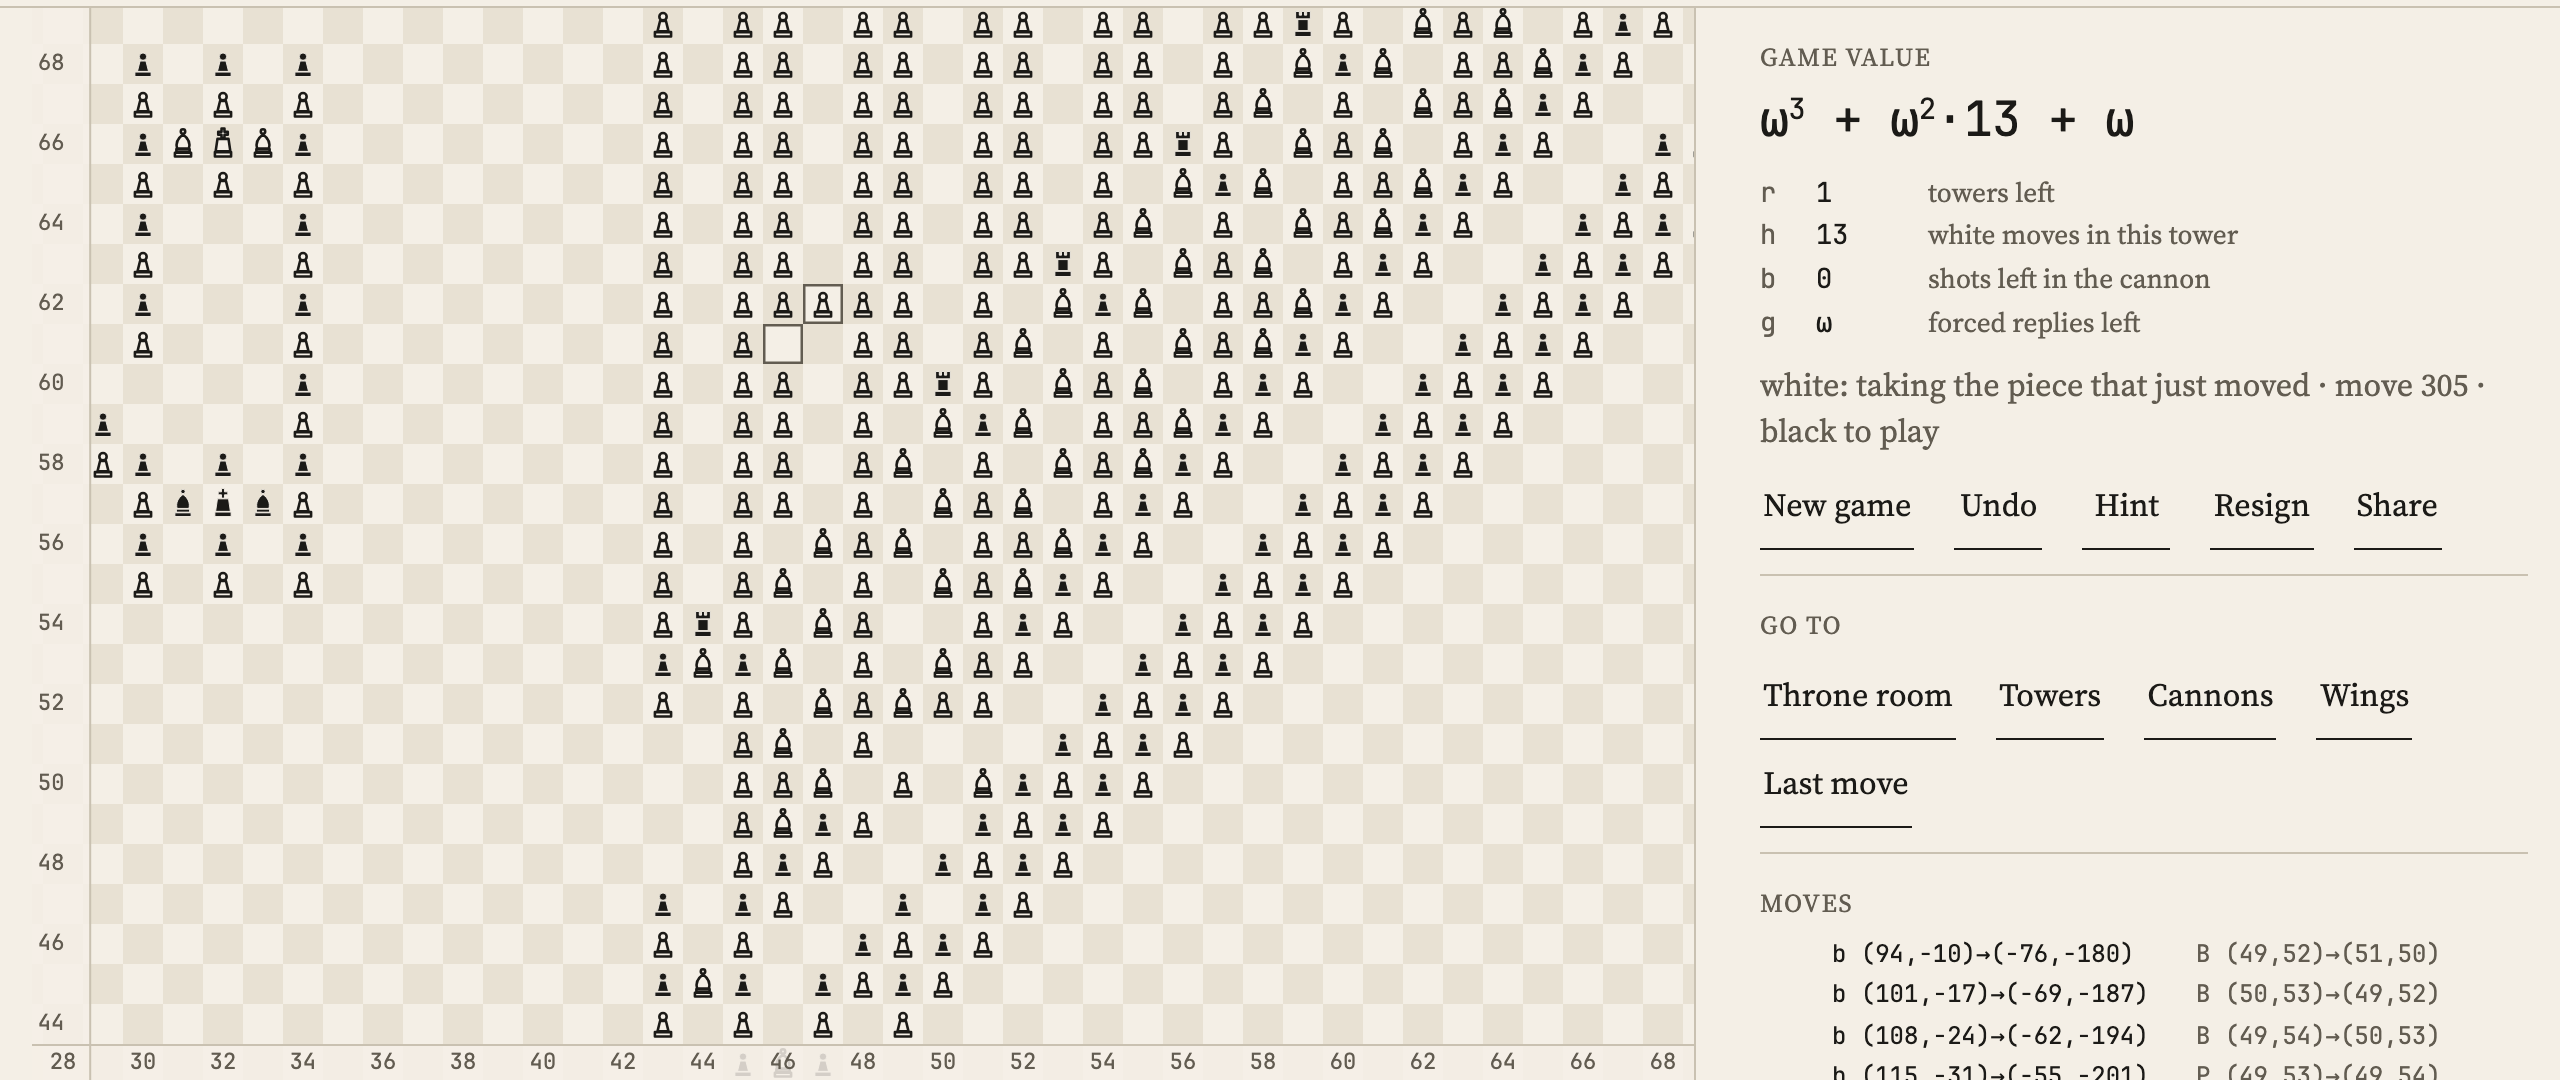
\includegraphics[width=\textwidth,height=0.67\textheight,keepaspectratio]{figures/demo/5-rook.png}
  \par\vskip 0.1cm
  {\footnotesize Before the lift the panel read $\omega^3\cdot 2+\omega$ with $h=0$. The height set $h$; the capture spent the tower and $r$ fell to 1.}
\end{frame}

\begin{frame}{Why deviations lose}
  \begin{description}
    \item[Bishop armies] Black could free extra bishops instead of firing them. They are penned in by the
      black-square pawn walls and can threaten only door pawns, which white answers as before.
    \item[Rook armies] Crazy rook moves in distant towers can be ignored in a fixed proportion, so they cost
      black more than the forced replies they replace.
    \item[Early exits] Leaving a gateway with the guard two behind loses the race by the tempo lemma.
    \item[White's side] No bishop can escape the towers early, and extra captures to the right only free
      useless bishops above the pawn diagonal.
  \end{description}
  \vskip 0.3cm
  \flag{proof sketch} each point is a one-line summary of a paragraph of \EHP, Section 3.
\end{frame}

\begin{frame}{The compact battery}
  \begin{columns}[T]
    \begin{column}{0.26\textwidth}
      \fig[\textwidth]{ehp17-fig6}
      \credit{Figure 6 of \EHP.}
    \end{column}
    \begin{column}{0.7\textwidth}
      Section 4 of \EHP\ folds the battery onto a quarter plane. The gateways stay as before; the cannons
      sit in a column with a vertical wall on the right. The same value formula applies, and the free quarter
      plane leaves room for larger constructions. The stills above come from this version.
    \end{column}
  \end{columns}
\end{frame}

\begin{frame}{Summary}
  \begin{itemize}
    \item Open games have ordinal values. A position has a value exactly when white can force a win, and
      the value measures how long black can delay. \flag{proved}
    \item Value $\omega$ is one announcement; $\omega^2$ nests announcements; $\omega^3$ nests again with
      towers. \flag{sketched from \EH}
    \item Replacing the harassing rook by a bishop cannon battery multiplies by $\omega^2$ instead of
      $\omega$, giving $\omega^4$. \flag{sketched from \EHP}
    \item Whether every countable ordinal is a value in ordinary infinite chess is open. \flag{conjecture}
  \end{itemize}
\end{frame}

\begin{frame}{References and credits}
  \scriptsize
  \begin{itemize}
    \item[\EH] C.~D.~A.~Evans and J.~D.~Hamkins, Transfinite game values in infinite chess,
      \emph{Integers} 14 (2014), \#G2. \url{https://doi.org/10.5281/zenodo.10454032}.
      Preprint arXiv:1302.4377v2 (24 February 2014), \url{https://arxiv.org/abs/1302.4377}.
    \item[\EHP] C.~D.~A.~Evans, J.~D.~Hamkins and N.~L.~Perlmutter, A position in infinite chess with
      game value $\omega^4$, \emph{Integers} 17 (2017), \#G4. \url{https://doi.org/10.5281/zenodo.10657427}.
      Preprint arXiv:1510.08155v1 (28 October 2015), \url{https://arxiv.org/abs/1510.08155}.
    \item[GS] D.~Gale and F.~M.~Stewart, Infinite games with perfect information, in
      \emph{Contributions to the Theory of Games II}, Annals of Mathematics Studies 28 (1953).
  \end{itemize}
  \vskip 0.3cm
  Board diagrams are the authors' own figures, typeset from their arXiv sources with the
  \texttt{chessboard} package; figure numbers follow the published versions.
  The demo and its source are at \url{https://github.com/sean-reid/infinite-chess}.
\end{frame}

\end{document}
